\chapter{Derivación de las condiciones de aceptabilidad}\label{AceppCon}

\subsection*{Sobre las funciones métricas}
\textbf{C1:} Las funciones métricas son positivas y deben ser finitas y libres de singularidades en el interior de la estrella.
\TODO{¿Razones físicas de esto?}
\subsection*{Condiciones de acoplamiento}\TODO{Verificar si de C3 se llega a continuidad de 1ra forma fund.}
 Para acoplar la solución interior y exterior sobre la superficie de la estrella, es necesario imponer condiciones de acoplamiento de modo que el espacio-tiempo este bien definido. 
 La formulación de estas condiciones usadas con mayor frecuencia fueron desarrolladas por Darmois\TODO{Cita.}\, y se basa en consideraciones sobre la curvatura intrínseca y extrínseca de la 3-superficie $\Sigma$ tipo tiempo que describe la superficie de la estrella.
 
 Si $\vec{n}$ es el vector (tipo espacio) normal a $\Sigma$, se introducen coordenadas Gausianas donde $n=cte$ define 3-superficies tipo tiempo vecinas a $\Sigma$ (ver Figura \ref{JC}). La métrica en estas coordenadas tiene la forma 
 \begin{equation}
g=(\vec{n} \cdot \vec{n})^{-1} d n\otimes d n +g_{i j} d x^{i} \otimes d x^{j}. 
\end{equation}

 \begin{figure}[H]
     \centering
     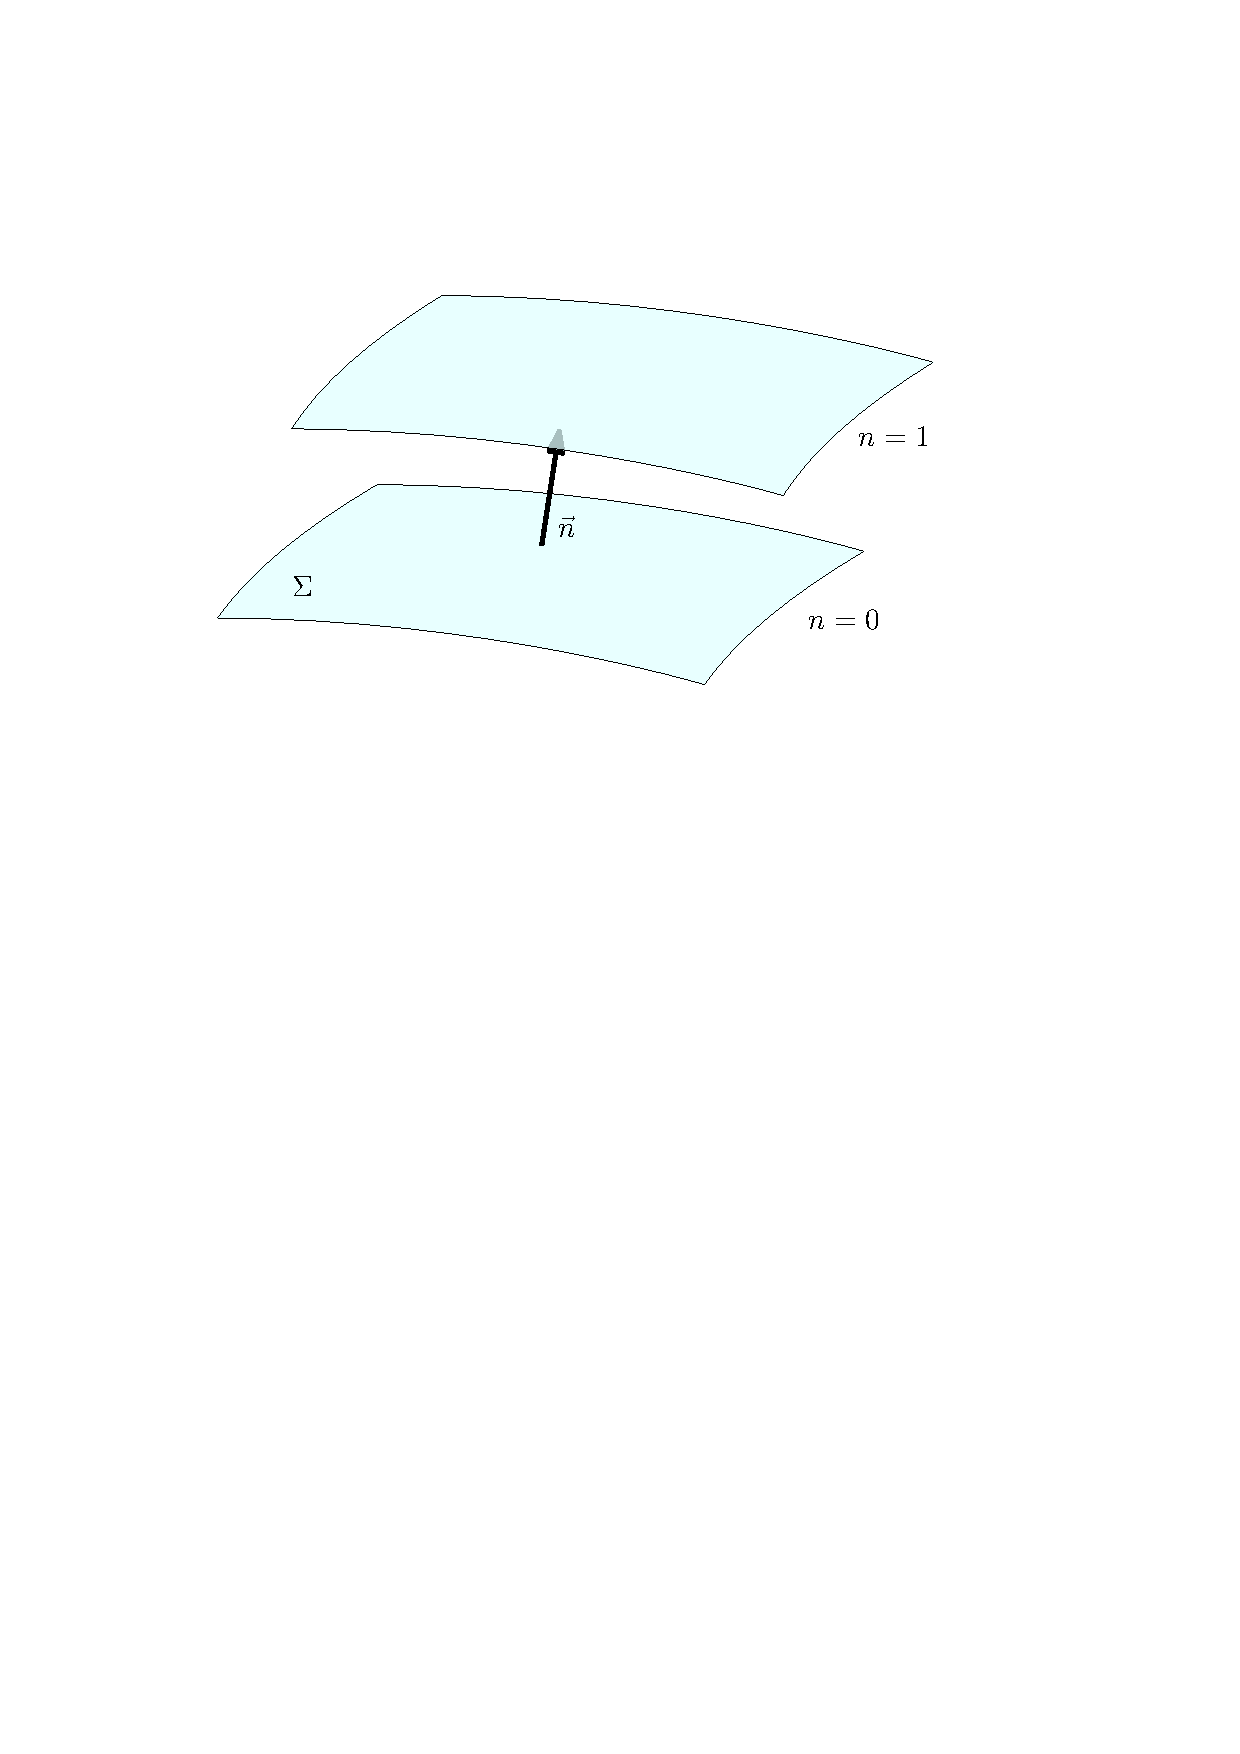
\includegraphics[width=0.7\linewidth]{figures/Junction.pdf}
     \caption{Coordenadas Gausianas en el vecindario a $\Sigma$}
     \label{JC}
 \end{figure}
Las condiciones de acoplamiento en este "set-up" son:
 \begin{enumerate}[leftmargin=2cm]
     \item La métrica inducida $g_{ij}$ es continua a través de $\Sigma$.
     \item El tensor de energía-momento superficial se anula en la superficie
     \begin{equation}
\lim _{\varepsilon \rightarrow 0}\left[\int_{-e}^{+\varepsilon} T_{\beta}^{\alpha} d n\right]=0.
    \end{equation}
     
 \end{enumerate}
 
 \textbf{C2:} Para el caso considerado en este trabajo $\Sigma:\,r=R$, además la simetría esférica permite identificar $\vec{n}=\pdv{r}$ y debido a que la solución externa es de vacío $\eval{T^{\alpha}_{\beta}}_{+\epsilon}$= 0, bajo estas condiciones las condiciones de acoplamiento se reducen a
 \begin{enumerate}[leftmargin=2cm]
     \item $e ^ {  2 \nu(R) } =  1 - \frac { 2 M } { R }$.
    \item $P(R)=\rho(R)=0$.
 \end{enumerate}


\subsection*{ Sobre el corrimiento al rojo gravitacional}
La luz emitida por una estrella es observada corrida al rojo por un observador lejano debido a la presencia del campo gravitacional. Qué tanto es corrida al rojo puede ser estimado de manera sencilla \cite{Glendenning2000}: considerando un átomo de la estrella a una distancia $r$ de su centro, que emite un fotones con determinada frecuencia, el intervalo de tiempo propio entre dos emisiones consecutivas está dado por
\begin{equation}
d \tau=\sqrt{-g_{\mu \nu} d x^{\mu} d x^{\nu}},
\end{equation}
en el marco del átomo esto es simplemente ($dx^i=0$)
\begin{equation}
d \tau_{\mathrm{e}}=\sqrt{-g_{00}(r)} d t.
\end{equation}
Si suponemos que el observador y el átomo yacen sobre la misma línea el intervalo espacio-temporal para la radiación es
\begin{equation}
d \tau^{2}=g_{11}(r) d r^{2} - g_{00}(r) d t^{2} = 0,
\end{equation}
así que el tiempo que tardó un ciclo en viajar de $r$ a $\infty$ es
\begin{equation}
\Delta t=t_{\infty}-t_{R}=\int_{R}^{\infty}\left(\frac{g_{11}(r)}{g_{00}(r)}\right)^{1 / 2} d r,
\end{equation}
es decir, $dt$ (tiempo coordenado entre dos emisiones consecutivas) es el mismo para el emisor y el observador lejano. Con lo anterior, el tiempo propio para el observador será
\begin{equation}
d \tau_{\mathrm{o}}=\sqrt{-g_{00}(\infty)} d t.
\end{equation}
Como el inverso del tiempo propio es proporcional a la frecuencia, la razón entre la frecuencia emitida y observada es
\begin{equation}
\frac{\omega_{\mathrm{e}}}{\omega_{\mathrm{0}}}=\left(\frac{g_{00}(\infty)}{g_{00}(r)}\right)^{1 / 2}=e^{-\nu(r)},
\end{equation}
y con esto el corrimiento al rojo gravitacional es
\begin{equation}
    z(r)\equiv \frac{\omega_{\mathrm{e}}-\omega_{\mathrm{o}}}{\omega_{\mathrm{o}}}  = e^{-\nu(r)}-1.
    \label{redshift}
\end{equation}
\textbf{C3:} El corrimiento al rojo descrito por \eqref{redshift} debe disminuir con el incremento de $r$.
\subsection*{Sobre el signo de la densidad de energía y la presión}
La densidad de energía y la presión deben ser positivas dentro de la estrella.\TODO{Materia normal?}

\subsection*{Sobre la densidad de energía y la presión}
\textbf{C5:} La densidad de energía y la presión deben alcanzar un máximo en el centro ($\rho'(0)=P'(0)=0$) y deben decrecer monótonamente hacia afuera.\TODO{Decrecimiento monótono?}

\subsection*{Condiciones de energía}
Con el fin de obtener soluciones a las ecuaciones de Einstein en presencia de fuentes de energía y momento realistas es necesario imponer ciertas condiciones de energía que limiten la arbitrariedad del tensor energía-momentum escogido.

Existe una variedad de condiciones de energía que son usadas en diferentes circunstancias, las usadas con mayor frecuencia son \cite{Hawking1973TheSpaceTime,Carroll2003SpacetimeRelativity}:

\begin{itemize}[leftmargin=1.5cm]
    \item \emph{Condición de energía débil}: el tensor de energía-momentum en cada punto $p$ de la variedad obedece la desigualdad $T_{\mu \nu} t^{\mu} t^{\nu} \geq 0$ para cualquier vector tipo tiempo $t^{\mu}\in T_{p}$.
    \item \emph{Condición de energía dominante}: el tensor de energía-momentum en cada punto $p$ de la variedad obedece la desigualdad $T_{\mu \nu} t^{\mu} t^{\nu} \geq 0$ y además $T^{\mu \nu} t_{\mu}$ es un vector que no es tipo espacio para cualquier vector tipo tiempo $t^{\mu}\in T_{p}$.
    \item \emph{Condición de energía fuerte}: el tensor de energía-momentum en cada punto $p$ de la variedad obedece la desigualdad $T_{\mu \nu} t^{\mu} t^{\nu} \geq \frac{1}{2} T_{\lambda}^{\lambda} t^{\sigma} t_{\sigma}$, para cualquier vector tipo tiempo $t^{\mu}\in T_{p}$.
\end{itemize}
Mientras que las condiciones débil y fuerte no se cumplen para el tensor energía-momento de algunos campos escalares con $m=0$ y $m\neq 0$ respectivamente \cite{Hawking1973TheSpaceTime}, la dominante es cumplida por todas las formas de materia conocidas y se requerirá por lo tanto que la materia en las estrellas de neutrones la cumpla. 

Escribiendo $t^\nu$ en una tétrada ortonormal $e_{\mu}$ como
\begin{equation}
    t^{\mu} e_{\mu}= \left(1+a^{2}+b^{2}+c^{2}\right)^{1 / 2} e_{0}+a e_{1}+b e_{2}+c e_{3},
\end{equation}
con el tensor de energía-momento de un fluido perfecto que se está considerando \eqref{EMT}, la condición $T_{\mu \nu} t^{\mu} t^{\nu} \geq 0$ se puede escribir como
\begin{equation}
T_{\mu \nu} v^{\mu} v^{\nu}=\left(1+a^{2}+b^{2}+c^{2}\right) \rho + \left( a^{2} +b^{2} +c^{2} \right) P \geq 0 \quad \forall a,b,c \in \mathbb{R},
\end{equation}
para el caso $a=b=c=0$ esto implica $\rho \geq 0$ y en el límite en que $a^2+b^2+c^2 \to \infty$ que $\rho + P \geq 0$.

Además, con $T^{\mu \nu} t_{\mu}$ escrito como
\begin{equation}
T^{\mu \nu} t_{\mu}e_{\nu}=\left(1+a^{2}+b^{2}+c^{2}\right)^{1 / 2} \rho e_{0}+a P e_{1}+b P e_{2}+c P e_{3},
\end{equation}
la condición de que no sea tipo espacio se convierte en
\begin{equation}
    -\rho^2 + (P^2-\rho^2)(a^2+b^2+c^2) \leq 0 \quad \forall a,b,c \in \mathbb{R},
\end{equation}
lo cual implica que $\rho \geq |P|$.

Debido a que en C1 se requirió que $\rho$ y $P$ fueran positivas, la condición de energía dominante añade la restricción $\rho \geq P$.

\textbf{C6:} La solución debe satisfacer la condición $\rho \geq P$.

\subsection*{Condición de causalidad}
El postulado de causalidad local en relatividad general prohíbe que alguna señal se propague a una velocidad mayor que la velocidad de la luz \cite{Hawking1973TheSpaceTime}. 

\textbf{C7:}  La velocidad del sonido en la estrella (modelada como un fluido) está dada por []\TODO{Usar una cita de algún libro de hidrodinámica}
\begin{equation}
    v^2=\dv{P}{\rho},
\end{equation}
y esta no puede sobrepasar la velocidad de la luz:
\begin{equation}
    0 < \dv{P}{\rho} \leq 1 .
\end{equation}
\REMARK{La presión y densidad son cantidades definidas localmente, así que la velocidad del sonido local debe ser menor a la velocidad de la luz.}

\subsection*{Criterio de estabilidad del índice adiabático }
\REMARK{$\Gamma=4/3$ para un gas polítropo relativista, pero este valor puede variar a lo largo de la estrella y ser menor. Las condiciones de estabilidad están dadas para el índice adiabático efectivo. Revisar con el profesor.}

\textbf{C8:} El índice adiabático debe satisfacer
\begin{equation}
    \Gamma = \frac { \rho + P  } { P } \dv{P}{\rho} \geq \frac{4}{3} \quad \text{WRONG}.
\end{equation}

\begin{equation}
     \langle\gamma\rangle=\frac{\int_{0}^{R} e^{(\lambda+3 \nu) / 2} \gamma(r) P(r) r^{2} d r}{\int_{0}^{R} e^{(\lambda+3 \nu) / 2} P(r) r^{2} d r},
\end{equation}

\begin{align}
    \gamma_{cr} = \frac{4}{3} +& \frac{1}{36} \frac{\int_{0}^{R} e^{(\lambda+3 \mathrm{v})}\left[16 P+\left(e^{\lambda}-1\right)\left(P+\rho c^{2}\right)\right]\left(e^{\lambda}-1\right) r^{2} d r}{\int_{0}^{R} e^{(\lambda+3 \mathrm{v}) } P r^{2} d r} \nonumber
    \\ &+ \frac{4 \pi G}{9 c^{4}} \frac{\int_{0}^{R} e^{(3 \lambda+3 \mathrm{v})}\left[8 P+\left(e^{\lambda}+1\right)\left(P+\rho c^{2}\right)\right] P r^{4} d r}{\int_{0}^{R} e^{(\lambda+3 \mathrm{v})} P r^{2} d r}
    \\ & + \frac{16 \pi^{2} G^{2}}{9 c^{8}} \frac{\int_{0}^{R} e^{(5 \lambda+3 v) }\left(P+\rho c^{2}\right) P^{2} r^{6} d r}{\int_{0}^{R} e^{(\lambda+3 v) } P r^{2} d r}. \nonumber
\end{align}
\subsection*{Estabilidad ante cracking}
El cracking es una posible inestabilidad de esferas autogravitantes ante perturbaciones locales.

\textbf{C9:} El criterio para que una distribución sea estable ante cracking presentada por Nuñez et al. \cite{Gonzalez2014CrackingSpheres} es
\begin{equation}
    0 \geq \dv{P}{r}.
\end{equation}

\subsection*{Estabilidad ante pulsaciones radiales. Criterio de Harrison-Zeldovich-Novikov}
Cuando se considera la estabilidad global de una configuraci\'on de energía con simetría esférica, se analiza cómo pulsaciones radiales pueden inducir el cuerpo a colapsar. 

\textbf{C10:} La estabilidad en este método estará determinada por la frecuencia del modo fundamental de oscilación (ver \cite{Haensel2007NeutronStructure,Shapiro1983}), sin embargo una condición más práctica para determinar si una configuraci\'on con simetría esférica es inestable globalmente es la conocida condición de Harrison-Zeldovich-Novikov, la cual enuncia que para una configuración sea estable respecto a oscilaciones radiales es \emph{necesario} que su masa $M$ aumente a medida que la densidad central $\rho_{c}$ crece: 

\begin{equation}
    \frac { \partial M \left( \rho _ { c } \right) } { \partial \rho _ { c } } > 0.
\end{equation}
Además, los puntos en los que $\frac { \partial M \left( \rho _ { c } \right) } { \partial \rho _ { c } } = 0$ (puntos críticos) son puntos donde la configuraci\'on pasa de estabilidad a inestabilidad.



\subsection*{Estabilidad ante convección adiabática}

La estabilidad contra convección se puede entender como sigue: cuando un elemento de fluido es desplazado hacia abajo, si su densidad aumenta más rápido que la densidad que lo rodea, el elemento se hundirá y la configuraci\'on será inestable. Por otro lado, si la densidad del elemento de fluido es menor que la de su alrededor, flotará y la estrella será estable contra convección.

\textbf{C11:} En el caso en que la perturbación del elemento de fluido es adiabática (pasa en intervalos de tiempo muy pequeños comparados con los del flujo de calor) Nuñez et al. \cite{Hernandez2018} mostraron que para que el modelo estelar fuera estable contra movimientos convectivos, el perfil de densidad $\rho(r)$ debe cumplir el siguiente criterio: 
\begin{equation}
    \rho ^ { \prime \prime } ( r ) \leq 0.
\end{equation}